\documentclass[fleqn,11pt]{olplainarticle}
% Use option lineno for line numbers 
\usepackage{graphicx} 
\usepackage{float} 
\usepackage{subfigure} 
\title{Pairwise Relationships Prediction System}


\author{Hanzhong Wang\thanks{1029740}}
\author{Xinnan SHEN\thanks{1051380}}
\author{Ziyue WANG\thanks{1014037}}

\affil{School of Computing and Information Systems, University of Melbourne}

\affil[]{\textit{\{hanzhongw,xinnan.shen, ziyue2\}}@student.unimelb.edu.au}


% \keywords{Keyword1, Keyword2, Keyword3}

% \begin{abstract}
% Please provide an abstract of no more than 300 words. Your abstract should explain the main contributions of your article, and should not contain any material that is not included in the main text. 
% \end{abstract}

\begin{document}
\maketitle
\flushbottom
\thispagestyle{plain}
\pagestyle{plain}


\section{Introduction}\label{intro}

\subsection{Background}\label{bgd}
\paragraph*{}
Pairwise Relationship is a very common relationship in our daily life. We can use pairwise relationships to store many forms of data, including the relationship between friends, the connections between devices in a network. In reality, when we build the pairwise relationships, it is inevitable that some edges between nodes are absent in the graph, which might mislead others a lot. Therefore, finding a way to predict the edges between nodes is an important step, as it makes the graph much closer to the reality. However, it is not an easy task to find all missing edges in a graph, as we don't know the real relationships between nodes. 
\paragraph*{}
In this project, we have implemented a system to predict the pairwise relationships between nodes by using machine learning tools. Given the nodes and some edges in the graph, the system can predict whether there is an relationship between them. The results have shown that the machine learning model works well in predicting the edges between nodes. Although there are some errors, the model still performs quite well.

\subsection{Related Works}\label{relaw}
\paragraph{}
Many researches related to pairwise link prediction have been conducted. For example, Liben-Nowell has created a relationship prediction model that can be used in social networks \citep{liben2007link}. Also, Zhou et al. have mentioned that they have adopted machine learning tools to predict the relationships between people \citep{lu2011link}. In our project, we will also use machine learning methods to make predictions. Meanwhile, some researchers believe that deep learning is a strong tool that can be used to predict relationships \citep{wang2019}, which has also been adopted in our model.
\paragraph*{}
In this paper, the system implementation details will be deeply discussed. In section \ref{datafeature}, we will discuss the method of extract training data from given dataset and the process of feature engineering. In section \ref{appres}, the approaches we have used to design the system and their corresponding results will be mentioned. In addition, section \ref{analysis} will analyse the possible error in this system and the causes of these errors. Finally, section \ref{conclu} will make a conclusion and state the possible improvements of this system.



\section{Data Sampling and Feature Engineering}\label{datafeature}

\subsection{Data Sampling}\label{data}
\paragraph*{}
The original training data “train.txt” contains 20,000 records of user-follow from Twitter, with a total of 4,867,136 nodes(users). Due to oversized experimental data, in this experiment, we only randomly selected 50,000 edges (source node, target node) from the original data as the true edges (positive sample) of the experimental training data, and randomly selected 50,000 edges (source node, target node)  that do not exist in the original training data as the false edges (negative sample) of the experimental training data. 

\subsection{Feature Engineering}\label{feature}
\paragraph*{}
In this project, the characteristics from the given training data can easily make us associate it with the graph, because the key of this task is belongs to the problem of link prediction. First, we preprocessed the data set because there are many irregular symbols or spaces. The preprocessing of the data ensures that the data is clean before tokenization. Second, we generate an undirected graph and directed graph based on the given training data. In this project, we created a new heuristic method to extract a feature. For example, if user M follows A, B, and C, and N is very similar to A, B, and C, we think M may follow N. In the project, we created M and N set that contains the item of A,B,C respectively, and then calculated the Jaccard similarity to measure the similarity between M and N.


\section{Approaches and Results}\label{appres}
\paragraph*{}
After we sampled data from the entire dataset and conducted feature engineering, we tried to use different kinds of machine learning tools to generate the results, including logistic regression, random forest and deep learning.

\subsection{Logistic Regression}\label{lr}
\paragraph*{}
Logistic Regression is suitable for binary classification problem, which we have treated as a baseline for this system \citep{menard_lr}. We have divided the processed data into training set and validation test \citep{scikit-learn}. To prevent the model from overfitting, we have used validation set not only to tune hyperparameters, but also to see the performance of the model in a very different dataset. Based on the performance of the model in the validation set, we have chosen the hyperparameters with the greatest accuracy to train the data and make predictions. The performance of Logistic Regression model can be seen as follows:

% table
\begin{table}[!htbp]
\centering
\caption{Logistic Regression Result}\label{tab:lr}
\begin{tabular}{ccc}
\toprule
Precision& Recall& F-1 Score\\
\midrule
0.99& 0.26& 0.41\\
\bottomrule
\end{tabular}
\end{table}
\paragraph*{}
From table \ref{tab:lr}, we can see that the logistic regression does not have a very good performance, but it is suitable to act as a baseline for this system.

\subsection{K-Nearest Neighbour}\label{knn}
\paragraph*{}
We have also used KNN classifier to try to improve the performance of the model \citep{Rebala2019}. Similar to what we have done in Logistic Regression, we have also divided the data into training set and validation set. By using scikit-learn tools \citep{scikit-learn}, we can train the model and predict the results more easily. Table \ref{tab:knn} has shown the results of K-Nearest Neighbour model. It is evident that KNN performs a little bit better than Logistic Regression, as the F-1 score is much higher. However, we still need to use some more powerful models to enhance the performance even further.

% table
\begin{table}[!htbp]
\centering
\caption{KNN Result}\label{tab:knn}
\begin{tabular}{ccc}
\toprule
Precision& Recall& F-1 Score\\
\midrule
0.62& 0.64& 0.63\\
\bottomrule
\end{tabular}
\end{table}



\subsection{Deep Learning}\label{dnn}
% TODO
\paragraph*{}
In this project, we have also used deep learning as a model to generate predictions. We have tried to use fully connected neural networks, and the activation function of output layer is sigmoid. The loss function is binary cross-entropy, which is suitable for binary classification problem \citep{tensorflow2015-whitepaper}. In particular, we have used the validation dataset to tune hyper-parameters so that we can select the model with the best performance to predict the final results.
\paragraph*{}
For DNN, we have tried models with 2, 3 and 4 hidden layers. The results is shown in figure \ref{fig:res}. From the graph, we can see that the performance of DNN has improved a lot, much better than Logistic Regression and KNN. In addition, the model with 2 hidden layers has the greatest F1-score in the validation set (82\%). Therefore, it performs best among all the models, and we have chosen this model to produce the final predictions.
\begin{figure}[H]
	\centering
	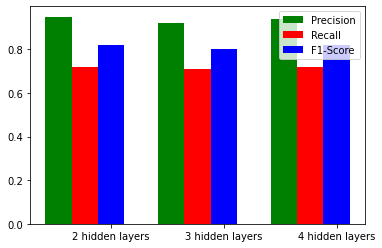
\includegraphics[scale=0.5]{result.png}
	\caption{Deep Neural Networks Result}
	\label{fig:res}
\end{figure}


\section{Critical Analysis}\label{analysis}
Thanks for using Overleaf to write your article. Your introduction goes here! Some examples of commonly used commands and features are listed below, to help you get started.

\section{Conclusion and Future Directions}\label{conclu}
\subsection{Conclusion}\label{con}
\paragraph*{}
Pairwise relationship is a useful relationship to store a number of data in real life. We have implemented a system to predict pairwise relationships, and the system can predict satisfactory results.
\subsection{Future Directions}\label{future}
\paragraph*{}
Although the system can generate satisfactory results, with high F1 score, its performance can be further improved.
\begin{itemize}
\item feature engineering: It is worth trying to generate more complex features from the training data to feed to the original model.
\item CNN: It is a good direction to consider Convolutional Neural Networks, as it might perform better than fully-connected neural networks.
\item Other ML tools: We could also try some other machine learning methods which we hadn't try in this project, like SVM.
\end{itemize}



\bibliography{sample}
% \printbibliograpy
% \small{*All contributions were made by all teammates equally in a comprehensive manner, and therefore it is hard to distinguish specific responsibilities}
\end{document}
